\section{Scripting}
\label{sec:script}

En SolTrace se pude utilizar scripts, ver Figura~\ref{fig:script}, para programar el trazado de rayos mediante \href{https://github.com/NREL/lk}{LK}. De esta manera es posible hacer simulaciones en lo largo del tiempo.


\begin{figure}[ht]
  \centering
  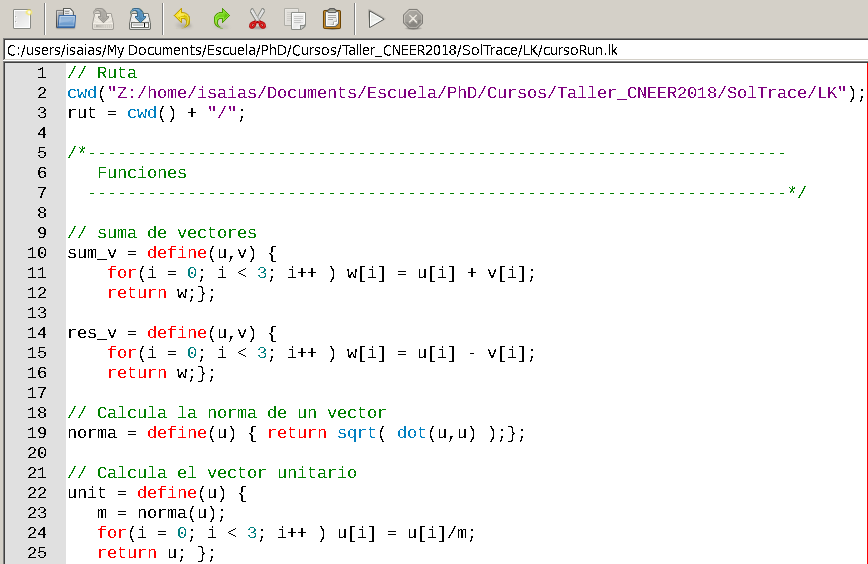
\includegraphics[width=1.0\textwidth]{figures/script}
  \caption{\label{fig:script} Script LK para la SolTrace.}
\end{figure}

El script LK es una modificación del lenguaje \verb=C=, puedes para conocer las característitcas básicas revisa el documento \href{https://github.com/NREL/lk/blob/develop/doc/lk_guide.pdf}{Guide LK}. A continuación se muestra un script para simular el helióstato del problema de la Sección~\ref{sec:helio}.


\lstinputlisting{./../LK/cursoRun.lk}

\section{Cálculo de la radiación solar}
\label{sec:radiacion}

Dado que el valor de la irradiancia varia con el tiempo, es necesario calcularla en el tiempo.


La radiación directa puede ser calculada, para diferentes horas y días, con un módelo de cielo claro~\citep{Dunham2013optical}, utilizando:

\begin{equation}
  \label{eq:DNI}
  G_b = G_0 \tau^{AM^{0.678}}
\end{equation}
donde $G_0$ es la constante solar de $1,367 \rm W/m^2$, y $\tau$ es la transmitancia atmosférica, que para condiciones de cielo claro tiene un valor de 0.7, y la masa de aire es obtenida como función de la altitud del lugar.
\begin{equation}
  \label{eq:AM}
  AM = \frac{ \exp(-0.0001184\,h_{\rm altitud})}{\cos \theta_z + 0.5057(96.080-\theta_z)^{-1.634}}
\end{equation}
$\theta_z$ es el ángulo cenital del vector solar, y $h_{\rm altitud}$ la altura sobre el nivel del mar.


%%% Local Variables: ***
%%% mode: latex ***
%%% TeX-master: "taller.tex" ***
%%% End: ***
